\documentclass[tikz,border=4pt]{standalone}
\usepackage{tikz}
\usetikzlibrary{arrows.meta}
\begin{document}
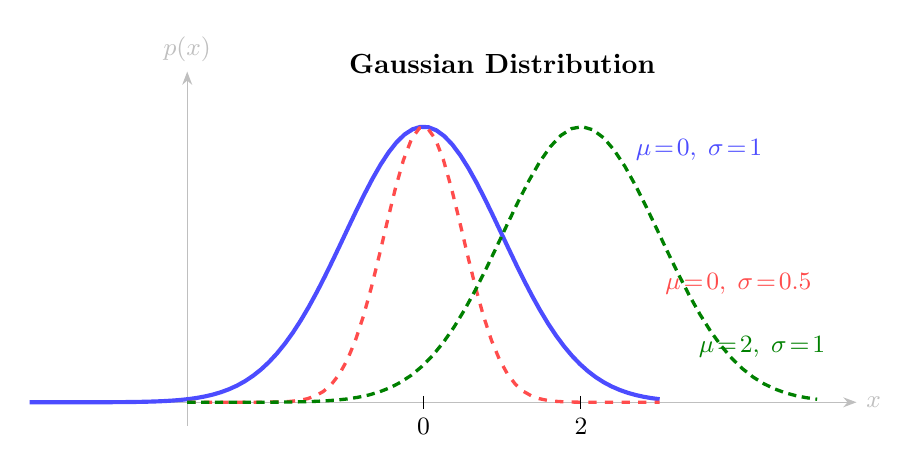
\begin{tikzpicture}[
    >=Stealth,
    axis/.style={->,gray!50},
]
\node[font=\bfseries] at (4,4.3) {Gaussian Distribution};

\draw[axis] (-0.5,0) -- (8.5,0) node[right,font=\small] {$x$};
\draw[axis] (0,-0.3) -- (0,4.2) node[above,font=\small] {$p(x)$};

% mu=0, sigma=1 (standard) - blue solid
\draw[blue!70,line width=1.5pt,domain=-2:6,samples=80]
    plot ({\x},{3.5*exp(-(\x-3)*(\x-3)/2)});

% mu=0, sigma=0.5 (narrow) - red dashed
\draw[red!70,line width=1.2pt,dashed,domain=0:6,samples=60]
    plot ({\x},{3.5*exp(-(\x-3)*(\x-3)/0.5)});

% mu=2, sigma=1 (shifted) - green dotted
\draw[green!50!black,line width=1.2pt,densely dashed,domain=0:8,samples=60]
    plot ({\x},{3.5*exp(-(\x-5)*(\x-5)/2)});

% Tick marks
\draw (3,0.08) -- (3,-0.08) node[below,font=\small] {$0$};
\draw (5,0.08) -- (5,-0.08) node[below,font=\small] {$2$};

% Legend
\node[blue!70,font=\small] at (6.5,3.2) {$\mu\!=\!0,\;\sigma\!=\!1$};
\node[red!70,font=\small] at (7,1.5) {$\mu\!=\!0,\;\sigma\!=\!0.5$};
\node[green!50!black,font=\small] at (7.3,0.7) {$\mu\!=\!2,\;\sigma\!=\!1$};
\end{tikzpicture}
\end{document}
